\begin{center}
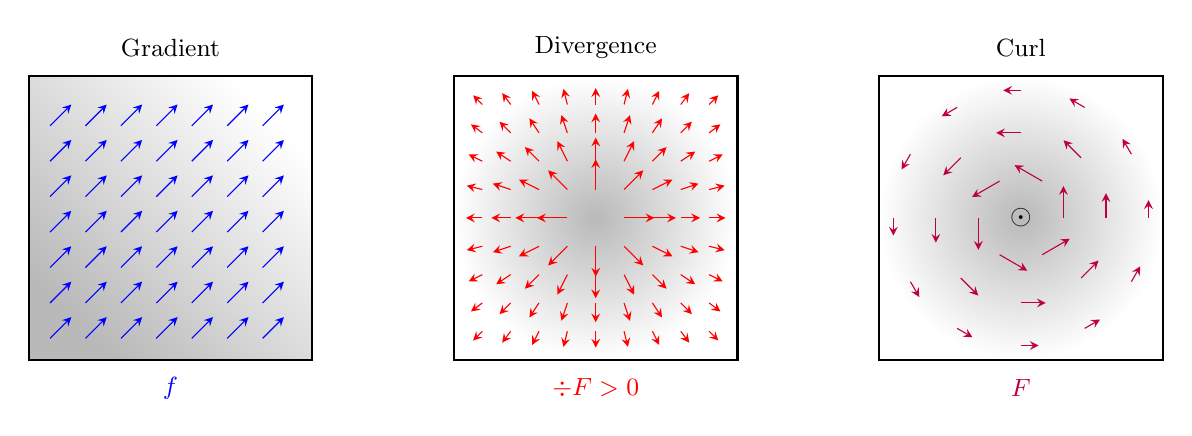
\begin{tikzpicture}[scale=0.9,>=stealth] 
    % Gradient panel 
    \begin{scope} 
        \shade[
            shading=axis,
            left color=gray!55,
            right color=white,
            shading angle=135
        ] (-2,-2) rectangle (2,2);
        \draw[thick] (-2,-2) rectangle (2,2);
        \node at (0,2.4) {\small Gradient};
        \foreach \x in {-1.7,-1.2,...,1.5} 
            \foreach \y in {-1.7,-1.2,...,1.5}
                \draw[->,blue] (\x,\y) -- +(0.3,0.3);
        \node[blue] at (0,-2.4) {\small $\grad{f}$}; 
    \end{scope}

    \begin{scope}[xshift=6cm]
        \shade[
            inner color=gray!55,
            outer color=white,
        ] (-2,-2) rectangle (2,2);
        \draw[thick] (-2,-2) rectangle (2,2);
        \node at (0,2.4) {\small Divergence};

        % Vector field
        \foreach \x in {-1.6,-1.2,...,1.7} {
            \foreach \y in {-1.6,-1.2,...,1.7} {

                % radius
                \pgfmathsetmacro{\r}{sqrt(\x*\x + \y*\y)}

                % avoid division by zero at center
                \ifdim \r pt > 0.05pt

                    % unit vector scaled by decaying function
                    \pgfmathsetmacro{\scale}{0.6/(1 + \r)}

                    \draw[->,red]
                        (\x,\y) --
                        ({\x + \scale*\x/\r}, {\y + \scale*\y/\r});

                \fi
            }
        }

        \node[red] at (0,-2.4) {\small $ \div{\vb{F}} > 0$};
    \end{scope}

    % Curl panel
    \begin{scope}[xshift=12cm]
        \shade[
            inner color=gray!55,
            outer color=white,
        ] (-2,-2) rectangle (2,2);
        \draw[thick] (-2,-2) rectangle (2,2);

        \node at (0,0) {$\odot$};

        \node at (0,2.4) {\small Curl};

        % Inner ring of circulation
        \foreach \a in {0,60,...,330}
            \draw[->,purple] (\a:0.6) -- +(\a+90:0.45);

        \foreach \a in {0,45,...,330}
            \draw[->,purple] (\a:1.2) -- +(\a+90:0.35);

        % Outer ring of circulation
        \foreach \a in {0,30,...,330}
            \draw[->,purple] (\a:1.8) -- +(\a+90:0.25);

        \node[purple] at (0,-2.4) {\small $\curl{\vb{F}}$};
    \end{scope}
\end{tikzpicture}
\textbf{Figure~\thefigure:} Visual depictions of a gradient of a scalar fuction (a), divergence of a vector function (b), and the curl of a vector function (c).
\label{fig:del}
\end{center}
